\chapter{Results and Discussion}
\section{Non-interactive segmentation performance}

After running the non-interactive segmentation evaluation of the models on the dataset, it was clear that \acs{mSAM} did not perform better than the classical baselines (see \cref{fig:dice_comparison} for a plot of the results).
The \acs{mSAM} model with the \acs{YOLO} box prompts performed particularly poorly, being the worst of all with a mean \acs{Dice} score of around \pgfmathprintnumber[fixed,precision=3]{\mSAMmean}.
At the same time, \acs{mSAM+pts} with the engineered point prompt clouds performed considerably better.
With a mean \acs{Dice} score of around \pgfmathprintnumber[fixed,precision=3]{\mSAMptsmean}, it performed comparably to the best performing classical baselines, \acs{Gaussian} and \acs{GC+brush} that each yielded \acs{Dice} scores of \pgfmathprintnumber[fixed,precision=3]{\Gaussianmean} and \pgfmathprintnumber[fixed,precision=3]{\GCbrushmean}, respectively.

The following subsections go into more detail on the results, and the statistical significance of the differences in performance between \acs{mSAM} and the classical baselines (see \cref{appendix:non-interactive-evaluation-data} in the appendix for the full results table).

\begin{figure}
\centering
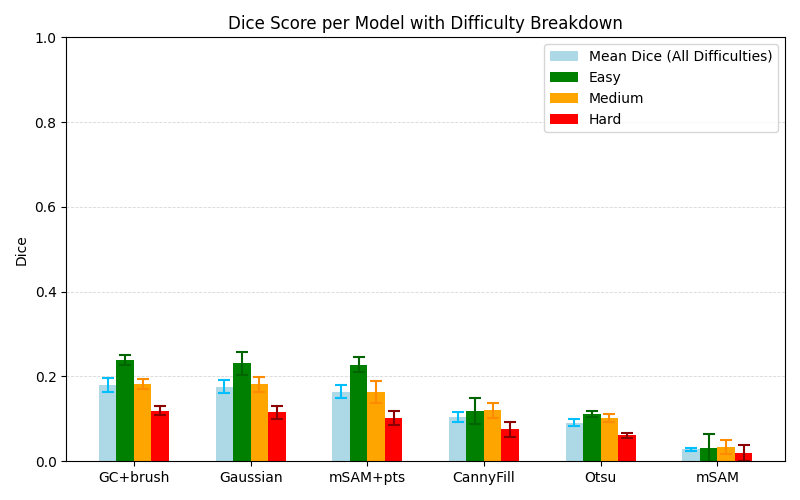
\includegraphics[width=\linewidth]{../src/data/plots/dice_score_comparison}
\caption{Dice Score performance per model. Split by difficulty. With error bars representing the standard error of the mean. Ordered descendingly from the left by mean performance.}
\label{fig:dice_comparison}
\end{figure}

\begin{figure}[htbp]
\centering
\begin{subfigure}{0.3\textwidth}
    \centering
    \fbox{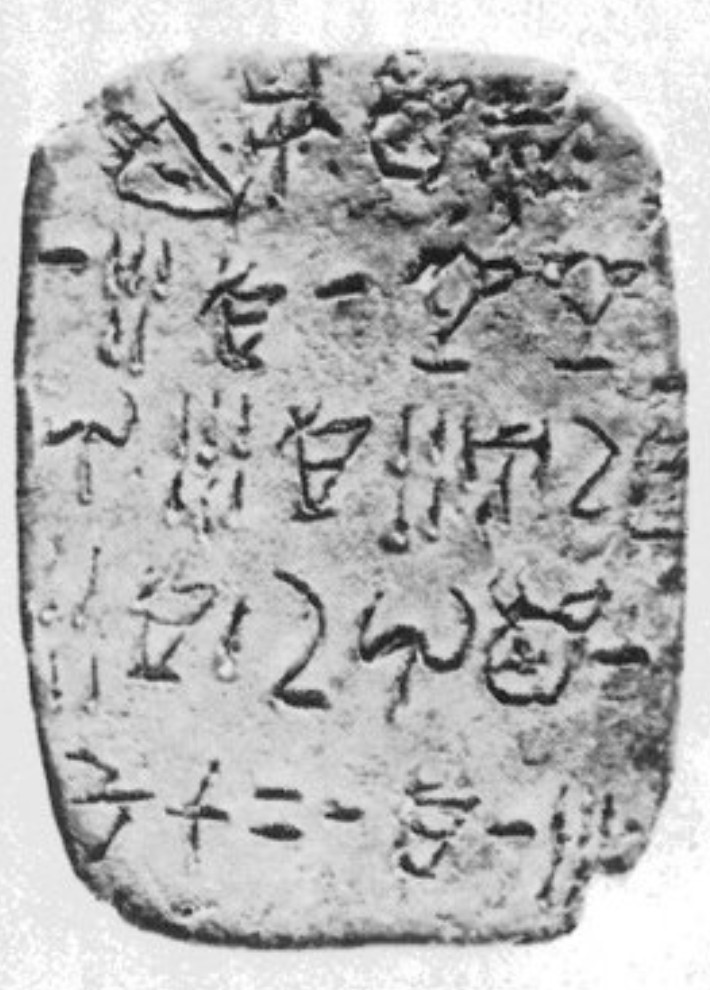
\includegraphics[width=\linewidth]{../src/data/raw/easy/HT118.jpg}}
    \caption{Raw Image}
\end{subfigure}
\hfill
\begin{subfigure}{0.3\textwidth}
    \centering
    \fbox{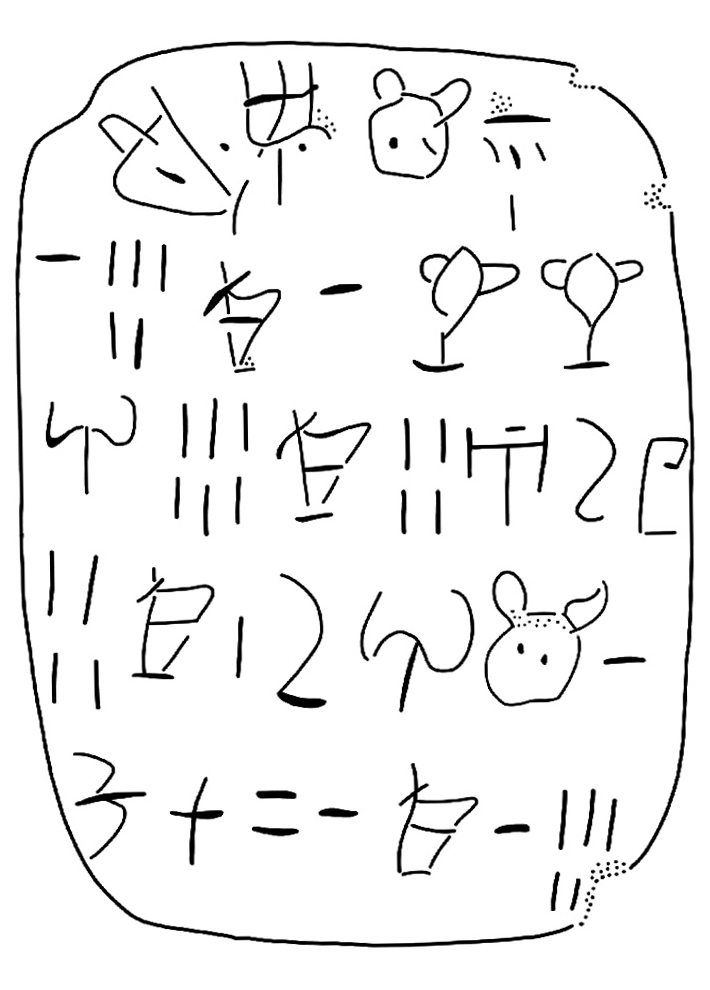
\includegraphics[width=\linewidth]{../src/data/ground_truth/registered/HT118.jpg}}
    \caption{Ground Truth}
\end{subfigure}
\hfill
\begin{subfigure}{0.3\textwidth}
    \centering
    \fbox{\includegraphics[width=\linewidth]{../src/data/scribed/HT118-Otsu.jpg}}
    \caption{Otsu}
\end{subfigure}
\vspace{0.5em}
\begin{subfigure}{0.3\textwidth}
    \centering
    \fbox{\includegraphics[width=\linewidth]{../src/data/scribed/HT118-Gaussian.jpg}}
    \caption{Gaussian}
\end{subfigure}
\hfill
\begin{subfigure}{0.3\textwidth}
    \centering
    \fbox{\includegraphics[width=\linewidth]{../src/data/scribed/HT118-CannyFill.jpg}}
    \caption{CannyFill}
\end{subfigure}
\hfill
\begin{subfigure}{0.3\textwidth}
    \centering
    \fbox{
\includegraphics[width=\linewidth]{../src/data/scribed/HT118-GC+brush.jpg}}
    \caption{GC+brush}
\end{subfigure}
\vspace{0.5em}
\begin{subfigure}{0.3\textwidth}
    \centering
    \fbox{\includegraphics[width=\linewidth]{../src/data/scribed/HT118-mSAM.jpg}}
    \caption{mSAM}
\end{subfigure}
\hspace{1em}
\begin{subfigure}{0.3\textwidth}
    \centering
    \fbox{
\includegraphics[width=\linewidth]{../src/data/scribed/HT118-mSAM+pts.jpg}}
    \caption{mSAM+pts}
\end{subfigure}

\caption{Visual comparison of output masks per model from segmentation on \acs{HT}118, shown next to the raw image and ground truth.}
\label{fig:model_comparison}

\end{figure}


\subsection{Statistical significance}

\subsubsection{Normality of residuals}

As the QQplot in \cref{fig:qqplot} shows, the residuals of the paired differences in \acs{Dice} scores between \acs{GC+brush} and \acs{mSAM+pts} appear to be approximately normally distributed, which supports the validity of the paired t-test results.
Furthermore, the Shapiro-Wilk test for normality on these residuals yields a p-value of $\pgfmathprintnumber[fixed,precision=3]{\ShapiroPValueResidualGrabCutSam} > \alpha = 0.05$, indicating that we fail to reject the null hypothesis of normality.

\begin{figure}[htbp]
    \centering
    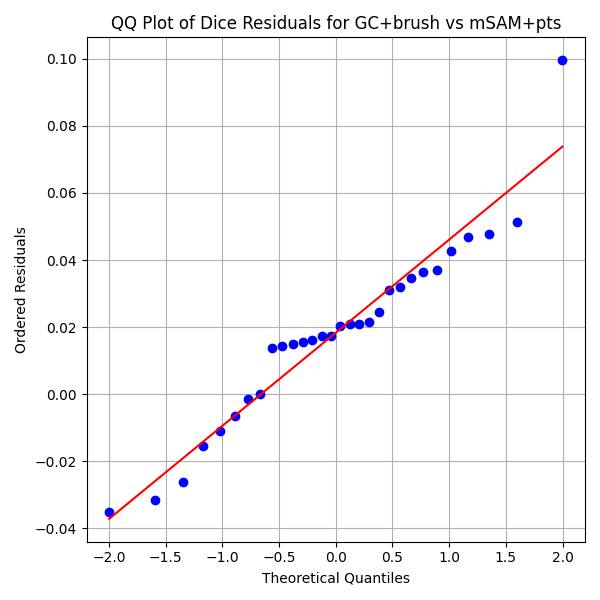
\includegraphics[width=\linewidth]{../src/data/qqplots/Dice_GC+brush_vs_mSAM+pts}
    \caption{QQplot of the residuals of the paired t-test comparing \acs{GC+brush} and \acs{mSAM+pts}. The residuals appear to be approximately normally distributed, which supports the validity of the paired t-test results. 
    Furthermore, the Shapiro-Wilk test for normality on these residuals yields a p-value of $\pgfmathprintnumber[fixed,precision=3]{\ShapiroPValueResidualGrabCutSam} > \alpha = 0.05$, indicating that we fail to reject the null hypothesis of normality.}
    \label{fig:qqplot}
\end{figure}

\subsubsection{Paired t-test}
To determine whether the classic baseline model \acs{GC+brush} signficiantly outperformed \acs{mSAM+pts}, a paired t-test is conducted on the \acs{Dice} scores obtained for each image across these two models.
The null hypothesis ($H_0$) states that there is no difference in mean \acs{Dice} scores between the two models, while the alternative hypothesis ($H_1$) states that \acs{GC+brush} has a higher mean \acs{Dice} score than \acs{mSAM+pts}.
Performing the paired t-test yielded the following results:
$$ \delta = \mu_1 - \mu_2 \approx \pgfmathprintnumber[fixed,precision=4]{\GCbrushmean} - \pgfmathprintnumber[fixed,precision=4]{\mSAMptsmean} = \pgfmathprintnumber[fixed,precision=4]{\deltameanGCmSAM} $$
$$ t \approx \pgfmathprintnumber[fixed,precision=3]{\tteststatGCmSAM} $$
$$ P(T > t) \approx \pgfmathprintnumber[fixed,precision=3]{\ttestpvalueGCmSAM} $$

Thus, as $\pgfmathprintnumber[fixed,precision=3]{\ttestpvalueGCmSAM} < \alpha = 0.05$, the null hypothesis can be rejected, and it can be concluded that \acs{GC+brush} significantly outperforms \acs{mSAM+pts} in terms of \acs{Dice} score.
Hence, it can be said that \acs{mSAM} underperforms in comparison to classical segmentation methods for one-shot segmentation of Linear A tablets, even when automatically prompted.

\section{Interactive segmentation performance}
\section{Workflow impact}